\section{\texorpdfstring{Control Web - Ovladače}{Control Web - Ovladace}}

% =====================================================================================================================
	\begin{frame}
    \frametitle{Ovladač}
		
		\begin{itemize}
			\item Je softwarová komponenta, která
			\item zajišťuje komunikaci mezi aplikací a konkrétním hardwarovým zařízením nebo komunikačním protokolem.
		\end{itemize}
		
		\vspace{5mm}
		\textcolor{blue}{\textbf{V kontextu Control Web}}
		
		\begin{itemize}
			\item zajišťuje komunikaci s HW, PLC nebo určitým SW objektem (virtuální generátor),
			\item mapuje proměnné z zařízení do proměnných v aplikaci,
			\item řeší detaily jako adresování (například TCPIP protokol), formát dat, časování komunikace.
		\end{itemize}

	\end{frame}
	
% =====================================================================================================================
	\begin{frame}
    \frametitle{Ovladač - výběr}
		
		\begin{center}
			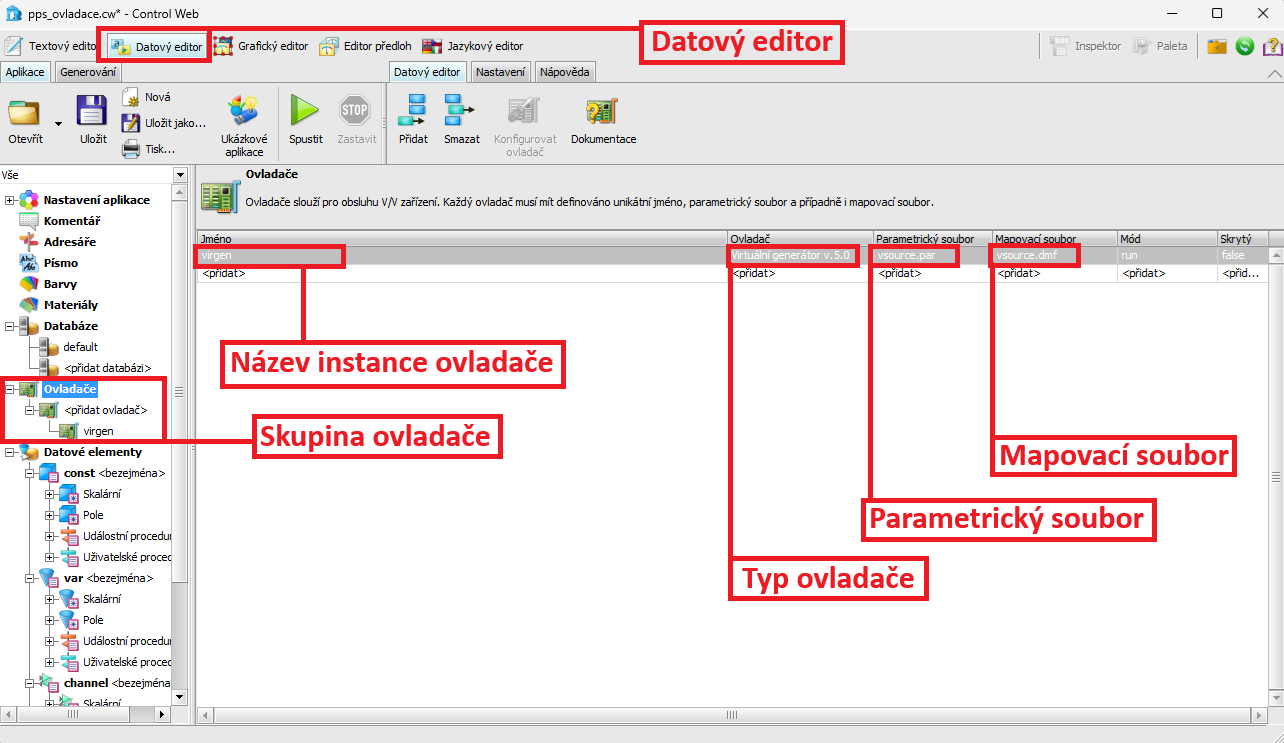
\includegraphics[width=1.00\textwidth]{fig/pridani_ovladace.png}
		\end{center}

	\end{frame}
	
% =====================================================================================================================
	\begin{frame}
    \frametitle{Parametrický soubor}
		
		\begin{center}
			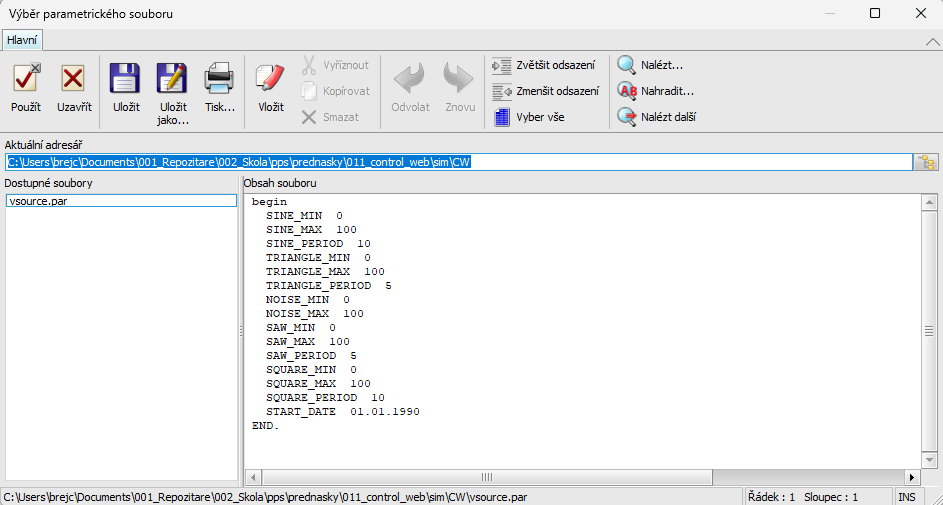
\includegraphics[width=0.80\textwidth]{fig/vyber_par.png}
		\end{center}
		
		\begin{itemize}
			\item soubor s konfiguračními parametry daného ovladače,
			\item různé ovladače mají různé druhy parametrů.
		\end{itemize}

	\end{frame}
	
% =====================================================================================================================
	\begin{frame}
    \frametitle{Mapovací soubor}
		
		\begin{center}
			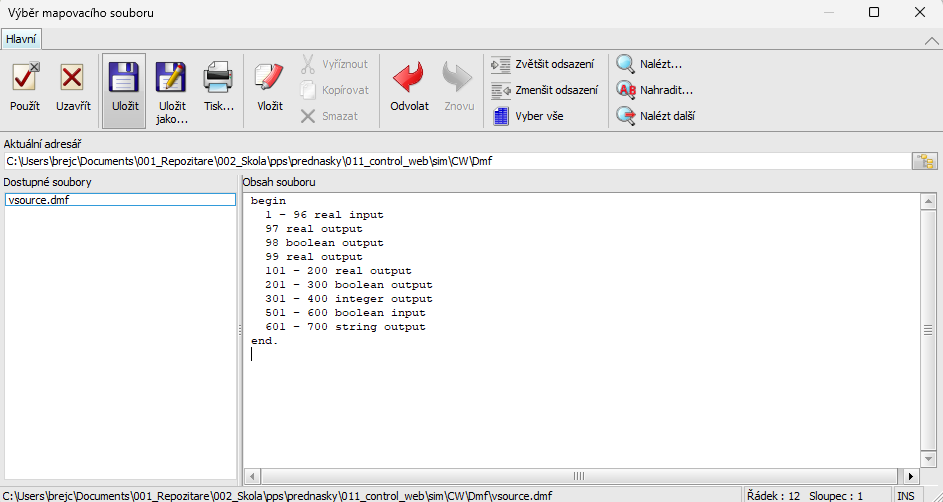
\includegraphics[width=0.80\textwidth]{fig/vyber_dmf.png}
		\end{center}
		
		\begin{itemize}
			\item soubor s definicemi kanálů ovladače,
			\item kanály nahrazují proměnné, používáme je pro zápis a čtení hodnoty. 
		\end{itemize}

	\end{frame}
	
% =====================================================================================================================
	\begin{frame}
    \frametitle{Seznam vyhrazených kanálů pro signály}
		
		\begin{minipage}[t][\textheight][t]{0.3\textwidth}
		
			\begin{enumerate}
				\item sinus,
				\item trojúhelník
				\item pila
				\item obdélník
				\item sinus
				\item trojúhelník
				\item šum
				\item pila
			\end{enumerate}

		\end{minipage}
		\begin{minipage}[t][\textheight][t]{0.6\textwidth}
		
			\begin{enumerate}
				\setcounter{enumi}{10}
				\item obdélník
				\item čas - počet sekund od půlnoci
				\item Juliánské datum
				\item počet dní od 1.1.1900
				\item rok
				\item měsíc
				\item den
				\item den v týdnu (1 až 7)
			\end{enumerate}
			
		\end{minipage}

	\end{frame}
	
% =====================================================================================================================
	\begin{frame}
    \frametitle{DMF a PAR pro instalaci doma}
		
		\begin{center}
			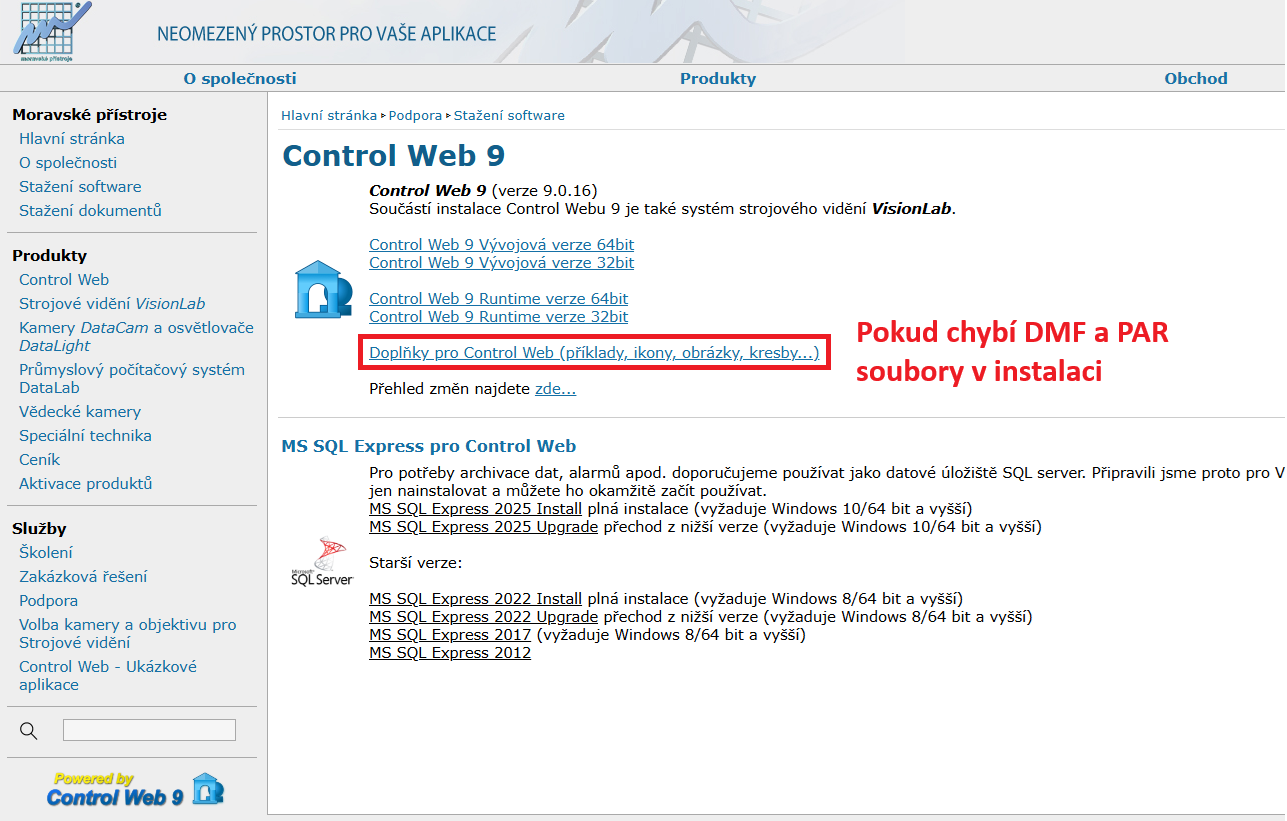
\includegraphics[width=0.90\textwidth]{fig/chybiovladace.png}
		\end{center}

	\end{frame}
	
% =====================================================================================================================
	\begin{frame}
    \frametitle{Přidání kanálu}
		
		\begin{center}
			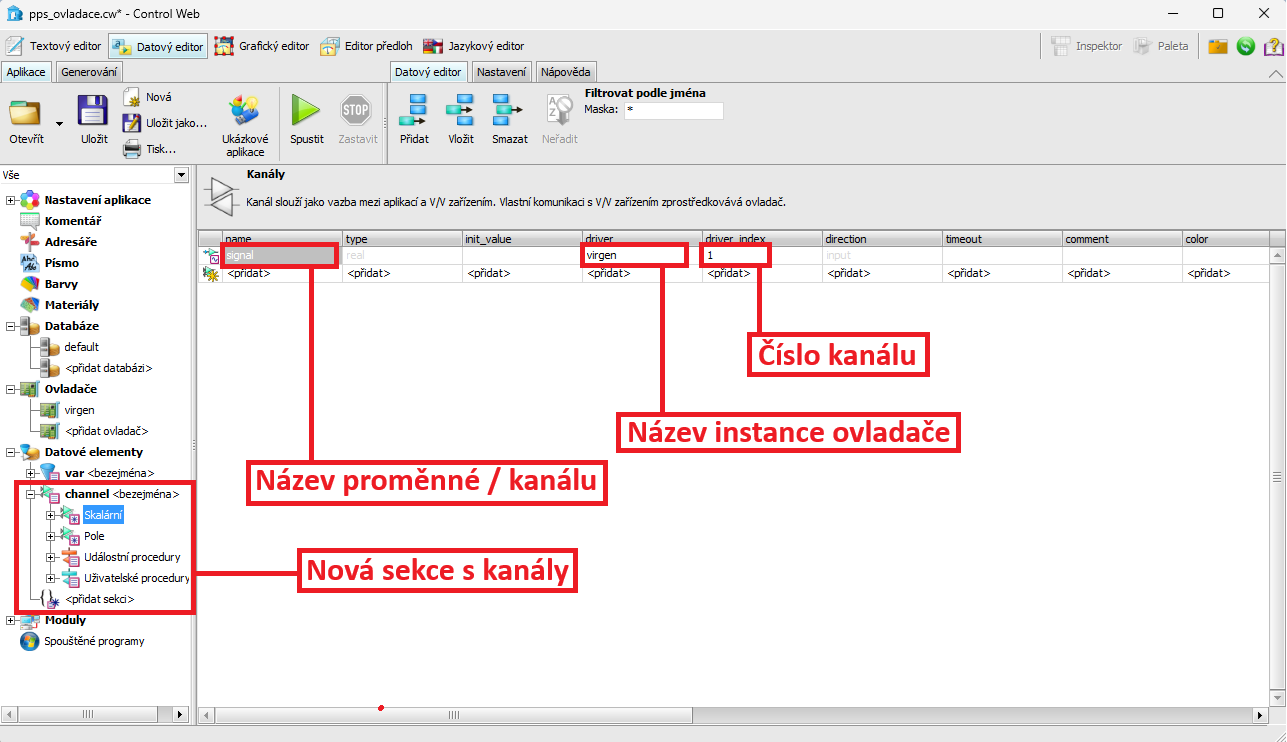
\includegraphics[width=1.00\textwidth]{fig/pridani_kanalu.png}
		\end{center}

	\end{frame}
	
% =====================================================================================================================
	\begin{frame}
    \frametitle{Návrh GUI}
		
		\begin{center}
			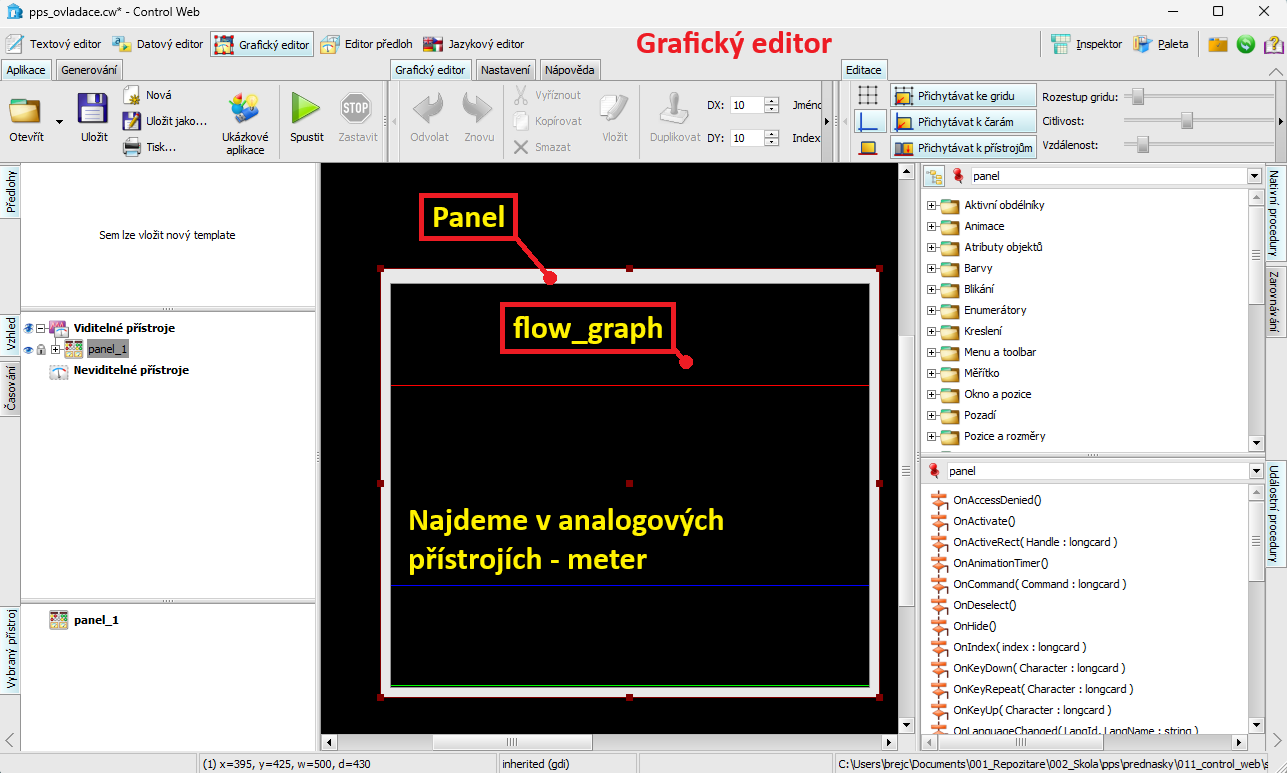
\includegraphics[width=1.00\textwidth]{fig/navrh_gui.png}
		\end{center}
		
	\end{frame}
	
% =====================================================================================================================
	\begin{frame}
    \frametitle{Připojení kanálu k přístroji}
		
		\begin{minipage}[t][\textheight][t]{0.55\textwidth}
		\small
		\textbf{Inspektor:}
		
			\begin{center}
				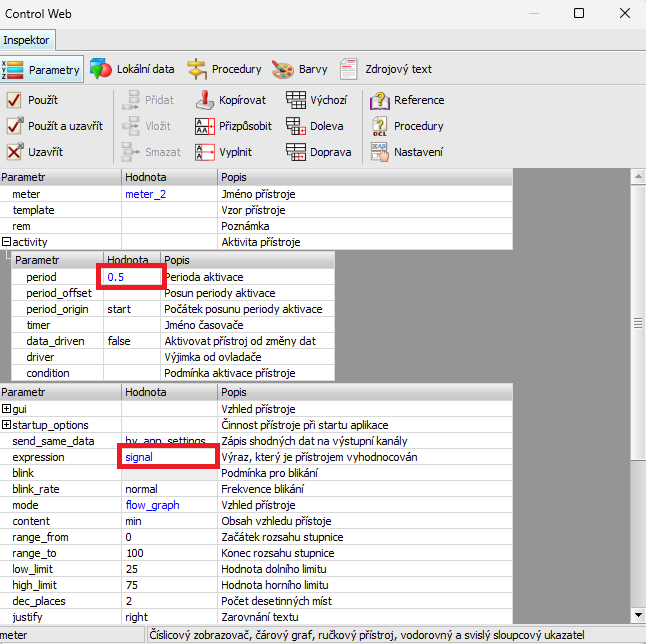
\includegraphics[width=1\textwidth]{fig/pripojeni_kanalu.png}
			\end{center}

		\end{minipage}
		\begin{minipage}[t][\textheight][t]{0.4\textwidth}
		
			\small
			\begin{itemize}
				\item Neliší se od proměnné,
				\item nastavujeme časování,
				\item do výrazu zadáváme kanál
			\end{itemize}
			
		\end{minipage}
		
	\end{frame}
	
% =====================================================================================================================
	\begin{frame}
    \frametitle{Aplikace po spuštění}
		\small
		\begin{center}
			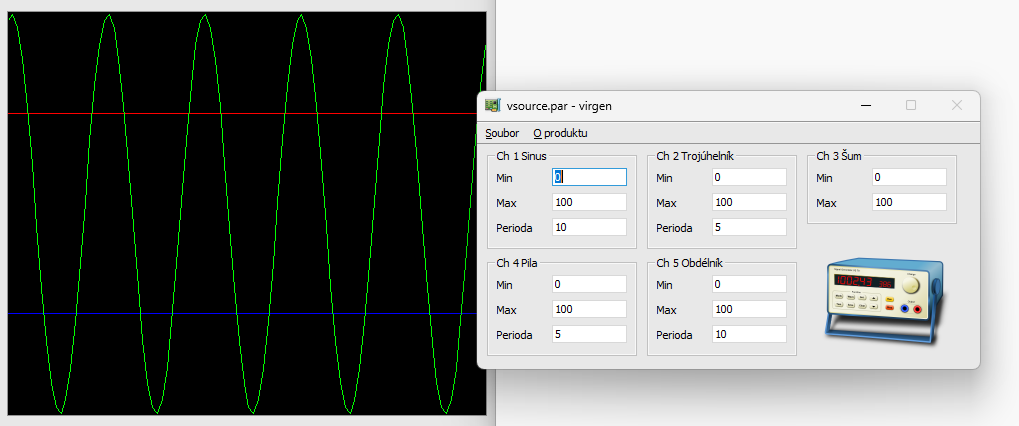
\includegraphics[width=1.00\textwidth]{fig/pps_ovladace_pred.png}
		\end{center}
		
		\begin{itemize}
			\item Okno parametrů generátoru se otevře při spuštění aplikace,
			\item během běhu aplikace lze měnit parametry kanálů 1-5.
		\end{itemize}
	\end{frame}
	
% =====================================================================================================================
	\begin{frame}
    \frametitle{Shrnutí}
		
		\begin{itemize}
			\item Ovladače zpřístupňují kontrolu HW nebo komunikace pro aplikaci,
			\item pro konkrétní situaci je nutný specifický ovladač:
			
			\begin{enumerate}
				\item \textcolor{blue}{\textbf{Ovladač CwNetDrv v.6.0}} - síťový přenos,
				\item \textcolor{blue}{\textbf{Ovladač ASCII v.7.0.8}} - sériová komunikace, ...
			\end{enumerate}
			
			\item parametry pro konkrétní ovladač jsou součástí \textbf{parametrického souboru},
			\item paměťový prostor (komunikační adresy kanálů) pro proměnné se definuje v \textbf{mapovacím souboru},
			\item v aplikaci kanál vystupuje stejným způsobem jako proměnná,
			\item kanály mají téměř vždy jen jeden druh přístupu pro zápis nebo čtení.
		\end{itemize}
	\end{frame}